%% ----------------------------------------------------------------
%% licenta.tex Fisierul principal
%% ----------------------------------------------------------------

\documentclass[a4paper, 11pt, oneside]{licenta}
\graphicspath{{Imagini/}}  % Folderul pentru imagini

% Pachete necesare
\usepackage[square, numbers, comma, sort&compress]{natbib}  % Folosim "Natbib" pentru bibliografie

% Macrouri
\newcommand\fhat{$F\hspace{4pt}\widehat{•}widehat{}\hspace{4pt}$}
\newcommand\frec{$F^{\emph{rec}}\hspace{2pt}$}
\newcommand\app{\hspace{2pt}}
%\newcommand\fixme[1]{ {\large \color[rgb]{1.0,0.0,0.0} \textbf{#1}} }
\newcommand\fixme[1]{#1}

%% ----------------------------------------------------------------
\begin{document}

\frontmatter	  % Numerotare cu cifre romane( i, ii, iii, iv...)
% Titlul lucrarii
\title  {Operational monitoring of ATLAS TDAQ evolution}
\fstsupervisor  {\texorpdfstring
            {\href{rd.hersch@epfl.ch} {Prof. R.D. Hersch}}
            {Prof. R.D. Hersch}}
            
\sndsupervisor  {\texorpdfstring
            {\href{wainer.vandelli@cern.ch} {Wainer Vandelli}} 
            {Wainer Vandelli}}

\authors  {\texorpdfstring
            {\href{ctalau@cern.ch}{Cristian T\u al\u au}}
            {Cristian T\u al\u au }
          }
\UNIVERSITY  {\texorpdfstring{\href{http://epfl.ch}
                {\' Ecole Polytechnique Fédérale de Lausanne - EPFL}}
                {\' Ecole Polytechnique Fédérale de Lausanne - EPFL}}
\faculty     {\texorpdfstring{\href{http://ic.epfl.ch}
                {School of Computer and Communication Sciences}}
                {School of Computer and Communication Sciences}}
% \addresses  {\groupname\\\deptname\\\univname}
\date       {\today}
\degree     {Master Thesis}
\subject    {}
\keywords   {}

\maketitle


%% ----------------------------------------------------------------

\pagestyle{fancy}  % Folosim titlul sectiunii in antetul paginii
\tableofcontents

%% ----------------------------------------------------------------
\mainmatter	  % Numerotare normala (1,2,3...)

% Capitolele lucrarii
\chapter{Introduction} % Titlul capotilului
\label{Capitolul1}

\section*{System Overview}
The LHC (Large Hadron Collider) is a 27km circumference synchrotron that accelerates two counter rotating particle beams. The beams are collided at four interaction points for a contiguous period of 10-20 hours. The ATLAS detector (A Toroidal LHC ApparatuS) \citep{aad2008atlas}, designed for studying particles produced by proton-proton interactions and heavy ion collisions surrounds one of the interaction points. 

The image below presents a section of the detector which has a layered structure with the interaction point in the center of the detector. The different layers are specialized in measuring different properties of the particles as detailed in \citep{aad2008atlas}. 

\begin{figure}[ht!]
\centering
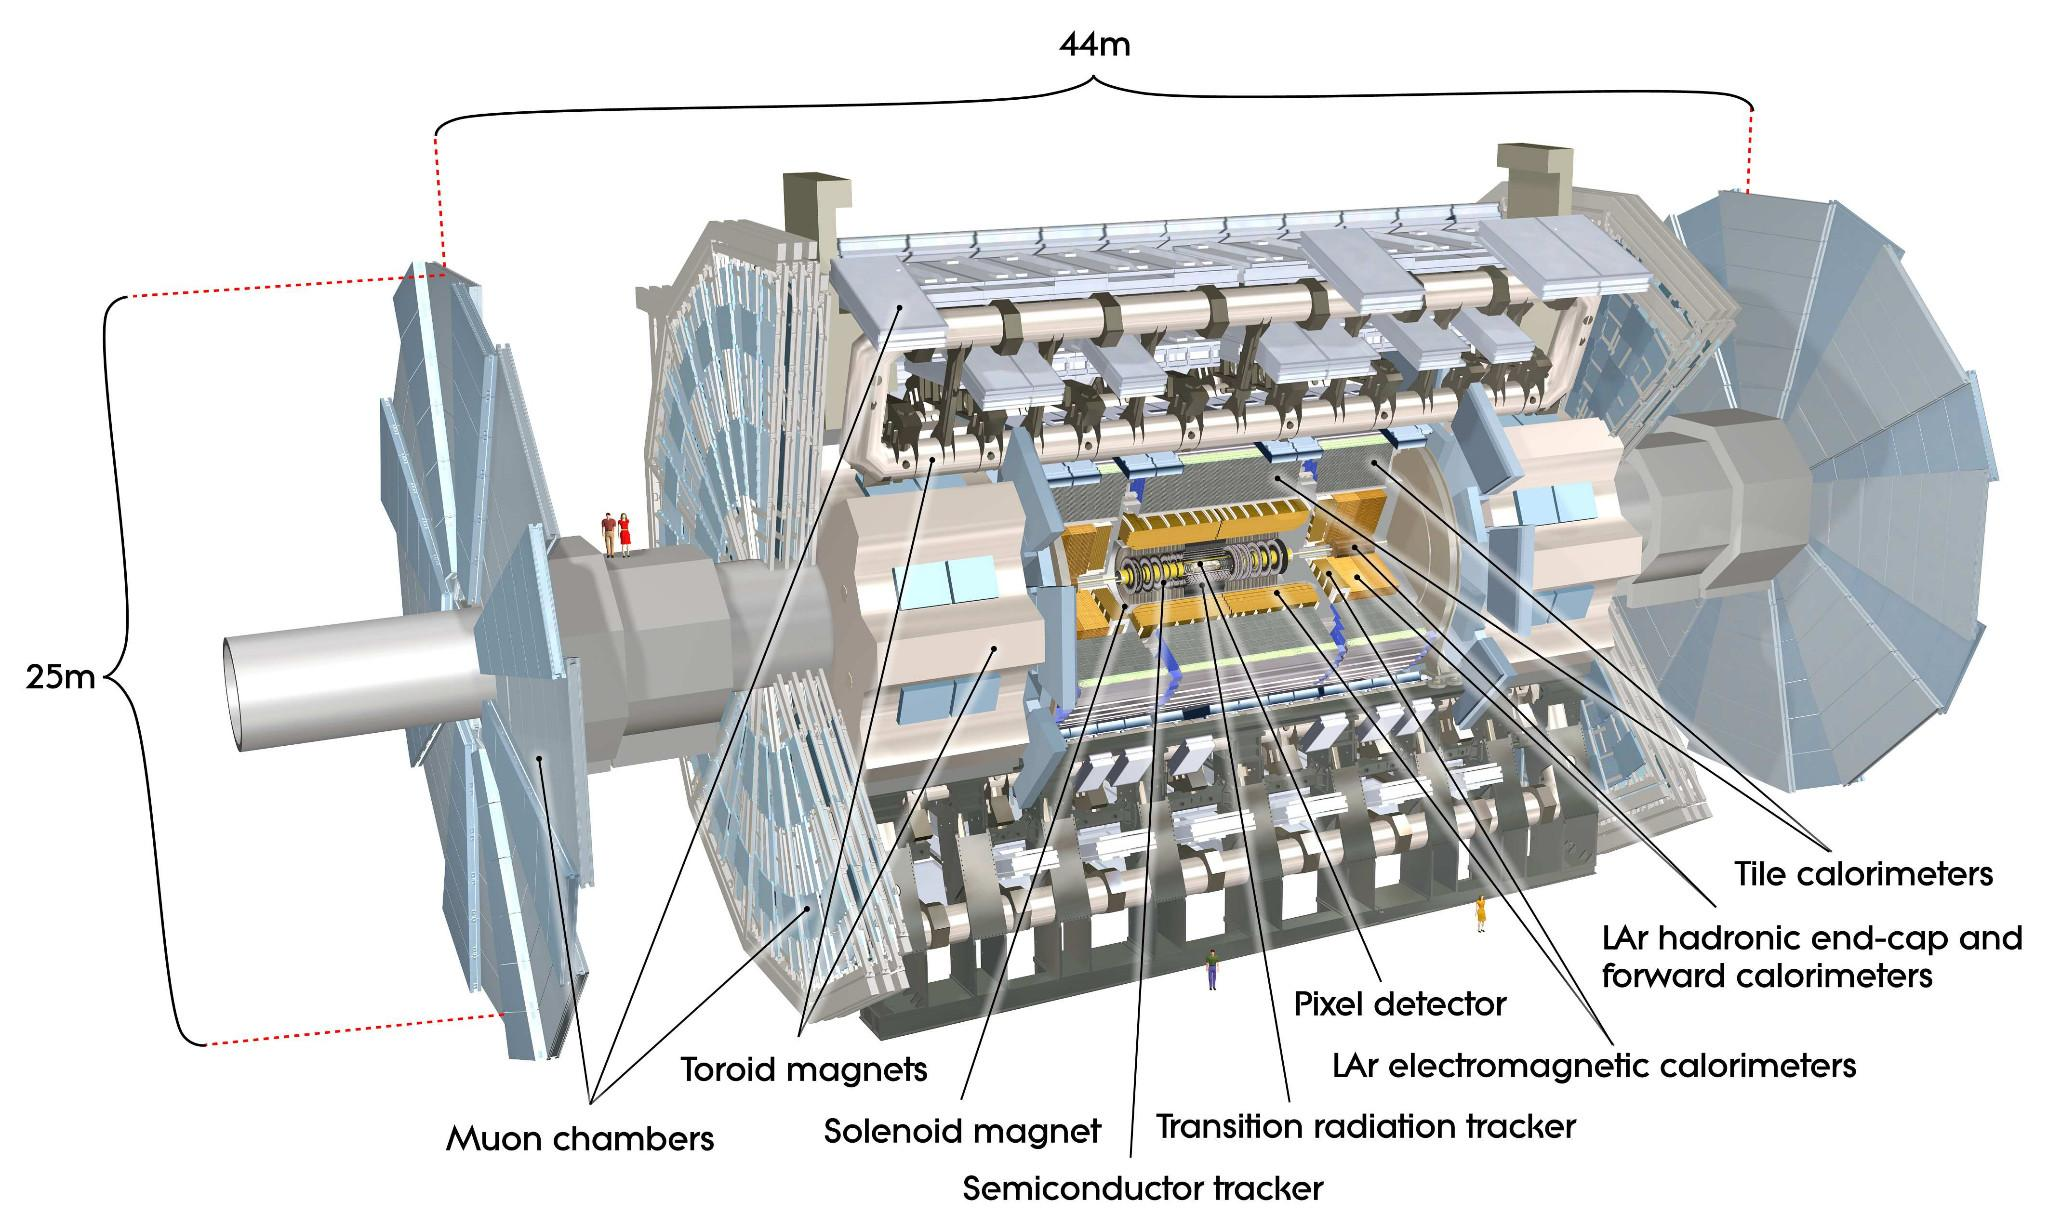
\includegraphics[scale=0.2]{Images/Overview.jpg}
\caption{ATLAS detector section view.}
\end{figure}


\section*{Event selection}
The two counter-rotating beams consist of trains of particle bunches. The distance between two consecutive particle bunches is around 25 ns and with the bunch crossing duration less than 1 ns. So bunch collision events happen with a frequency of 40MHz, each one consisting of 25 particle collisions in average. The data collected about these collisions has to be sent to the CERN persistent storage \citep{baud2003castor} for offline analysis. The amount of data collected for a single collision event is 1.5MB in average, which would mean a throughput of 60TB/s which is far more than what can be stored at a reasonable cost. Moreover, the number of events that are interesting for the offline analysis is only a small fraction of the total number of events. Hence, the events are filtered before being persisted using a three level data acquisition system (DAQ). 

\begin{figure}[ht!]
\centering
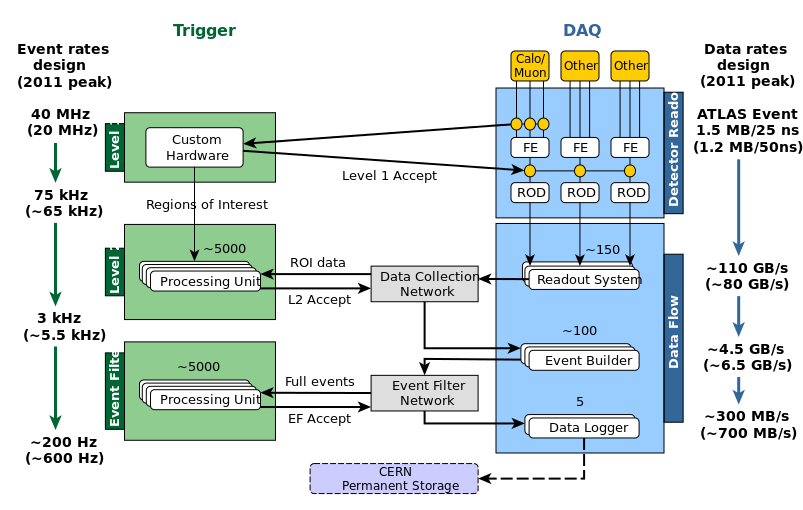
\includegraphics[scale=0.5]{Images/Trigger.png}
\caption{TDAQ system overview.}
\end{figure}

The first level trigger (L1) is built using custom hardware that can operate at 40 MHz and is placed as close to the actual detector as possible to reduce latencies caused by cable length. This level makes simple decisions based on the energy depositions in the calorimeters and of muon track segments in order to limit the latency to as low as 2.5 us. The acceptance rate of this level is chosen to be at most 75kHz. 

After being accepted by the L1, event data is stored in the ROBs (ReadOut Buffers) while it is processed by the second level trigger (L2) which is part of the HLT (High Level Trigger). The L2 reads only some parts of the data associated with an event (Regions of Interest or ROI) as hinted by the L1. The data used by the L2 system is in average 50KB per event and the latency of the order of tens of milliseconds. The L2 selection software is composed of more than 6000 instances of a software application running on 800 nodes, each of them handling one event at a time. 

Finally, the third level trigger, called Event Filter (EF) operates on the complete event data, at an input rate given by L2 of 3.5kHz. It has a configurable menu of more complicated selection algorithms and has a total latency of about 1 seconds and an acceptance rate of several hundred hertz which is within the mass storage limitations. The installation consists of 600 nodes running 6500 instances of the applications.

\subsection*{Evolution}

During the 2 year shutdown period starting at the beginning of 2013, a large upgrade of the entire system is planned \citep{hauser2012atlas}. In the DAQ system, the main change will be the merge of the L2 and EF.  

\begin{figure}[ht!]
\centering
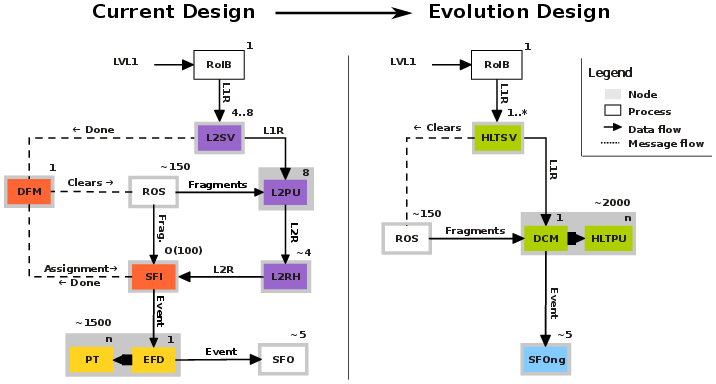
\includegraphics[scale=0.55]{Images/Evolution.png}
\caption{ATLAS TDAQ architecture evolution during shutdown.}
\end{figure}

All the applications dealing with event dispatching and other system management and control tasks (DFM, SFI, L2RH, EFD) will be merged into the HLT SuperVisor (HLTSV) and the DataFlow Control Manager (DCM). 
The L2 Processing Unit (L2PU) and the level 3 processing task (PT) will be merged into the HLTPU. In the new system instead of having L2 operating on chunks of event data and EF on whole events, we will have a series of algorithms that fetch event chunks incrementally as needed.

The main advantages of merging the two layers are better resource allocation, better load balancing and a simpler and more flexible system. However, assessing the benefits of this change needs validation in production mode with intensive operational monitoring.

\section*{Monitoring in ATLAS}

The ATLAS monitoring system \citep{collaboration2003atlas} is composed of information publishing libraries, information sharing services, monitoring facilities (e.g. that aggregate or persist monitoring information) and graphical displays.

There are two types of monitoring: operational monitoring which deals with operational data and functional parameters of different software and hardware components and event monitoring which monitors results of the analysis performed on events.

\subsection*{Components and services}

There are a number of components and services that play together in the monitoring system. We will present below the ones that have are the most relevant for operational monitoring starting from the lowest level ones up.

\begin{description}
\item[Inter-Process Communication (IPC) library \citep{corso2007data}] Is responsible for all the communication between applications in the ATLAS Trigger and Data AcQuisition (TDAQ)  system. It provides a much simpler interface to the underlying CORBA implementation including a simple API for the OMG Naming Service and a transparent cache for the remote object references.

\item[Object Kernel Support (OKS) database \citep{jones1998oks}\citep{alexandrov2001atlas}] Is an object-oriented database used for storing static configuration parameters for hardware and software components of the system, for example command line parameters and the node where to run a specific application. The data is loaded from XML data files and is validated against an user provided schema. 

In order to avoid overloading the database server during the system start and due to the static nature of the data, a system of caching proxies is used. This and the fact that the database does not have advanced query support enables it to meet the performance requirements of a real-time system.

\item[Partition editor] The software and hardware components in the TDAQ system are grouped in partitions which are configured using an OKS database. Due to the scale of the partitions (e.g. hundreds of applications), the configuration cannot be specified manually, but is automatically generated using a set of tools called partition editor.

\item[The ROOT framework \citep{brun1997root}] is an Object Oriented framework that contains among others an efficient file-based persistence mechanism, a C++ interpreter, reflection support, advanced statistical analysis instruments (multi dimensional histograms, fitting, minimization) and visualization tools. Most of the monitoring information in the system consists of such histograms.

\item[Information Sharing (IS) server \citep{kolosinformation}]  Is a server used to share monitoring information between applications that publish their own operational or event-related data and applications that need to process this information. The IS acts as an in memory key-value store, where keys are strings - the name of the objects - and values are subclasses of the ISInfo class. An application can read, write or update the information with a specific name. There is also the option for an application to subscribe to receive notifications when a value is updated. Due to the scale of our system, we run multiple instances of this server, each having its own name.

\begin{figure}[ht!]
\centering
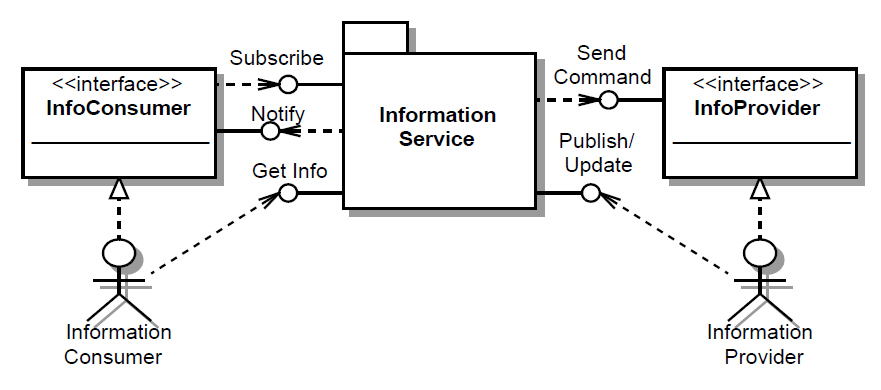
\includegraphics[scale=0.44]{Images/IS.png}
\caption{IS server interface.}
\end{figure}


The ISInfo class is intended to be a plain data structure with serialization and deserialization functions. They can be either written by the programmer or generated from an XML description.

\item[The Online Histogramming (OH) service \citep{kolosoh}] is a library which offers an interface to the IS server that allows one to store and retrieve ROOT histograms by transparently encoding them as ISInfo objects.

\item[The Gatherer \citep{renkel2010gatherer}] Is an application which aggregates monitoring information coming from different applications. For example, many applications track event data size distribution using histograms. The gatherer periodically reads all these histograms from the IS server, adds them and writes them back to the IS server. The aggregation is usually done in multiple stages, once per rack, and once globally across different IS servers. 

\item[Persistent Back-End for the AtlaS Tdaq (PBEAST) \citep{sicoe2012persistent}]: A Java application that persists operational monitoring data while storing the most recent data (1 month) in a queryable format. It subscribes to most of the IS servers and stores the updates in a Cassandra database.

\end{description}

\section*{Thesis structure}

The rest of the thesis report begins with a presentation of the project goal, namely the design and implementation of the {\tt monsvc} library. Then we describe the solutions for the challenges related to the \emph{configuration} of the library. In the next section, we present the algorithm used to \emph{schedule} the flow of monitoring information in the TDAQ network. Finally, we discuss some solutions for the \emph{synchronization} between the library which publishes the monitoring information and the application that updates it. The thesis ends with conclusions and possible future improvements.



\chapter{The {\tt monsvc} library} % Titlul capotilului
\label{Capitolul2}

The goal of my master project is to implement a library used by the applications to publish monitoring information to the IS servers \citep{kolosinformation}. This section is a brief overview of the functionality of the library. The following sections will present more details about specific aspects of the implementation such as configuration, scheduling and synchronization.

A data taking session of an LHC production fill lasts between 10 and 20 hours. During this time it is important to be able to monitor different operational parameters of the ATLAS TDAQ system and to react to abnormal conditions. For example, one needs to readjust parameters of the event selection software if the acceptance rate becomes so high that persistence services cannot handle it. 

To this end, all the applications in the system need to provide real-time updates about their operational conditions. These updates consist of (multidimensional) histograms, counters, rates, boolean variables, strings and collections thereof - we will refer to them as \emph{monitored objects}. Some examples of such objects are a counter of wrong checksums for event data read from the L1 filter or a histogram of the event sizes for the events accepted by the L2 filter. The updates are sent either periodically, or on demand: at the end of the run, when some exceptional condition occurs or when requested by the operator.

The {\tt monsvc} library takes care of the periodic publication of the monitored information, completely abstracting this task and leaving the application programmer in charge of solely updating the information with the current operational values. This is beneficial since the monitoring information is updated more often and more irregularly than it is published. For example, the counter of wrong checksums is updated every time such an error occurs, but it is expected to be published every 5 seconds. The interval between two publications of a monitored object is called call publishing interval.

In the monsvc approach, the monitoring is split into two operations: registration and publishing. The registration consists of passing a reference to an object to be monitored together with a name for that object to the monsvc library. The publishing deals with sending the data periodically to an IS server from where other applications will read it and either present it to the user or take corrective actions upon failures. 

The programmer needs to register the monitored objects (via the {\tt MonitoringService}), to configure the publishing process and to start it (via the {\tt PublishingController}). After this the programmer just needs to update the registered objects to reflect the current operational values. The image below presents an example workflow that the user may employ when working with the library.  

\begin{figure}[ht!]
\centering
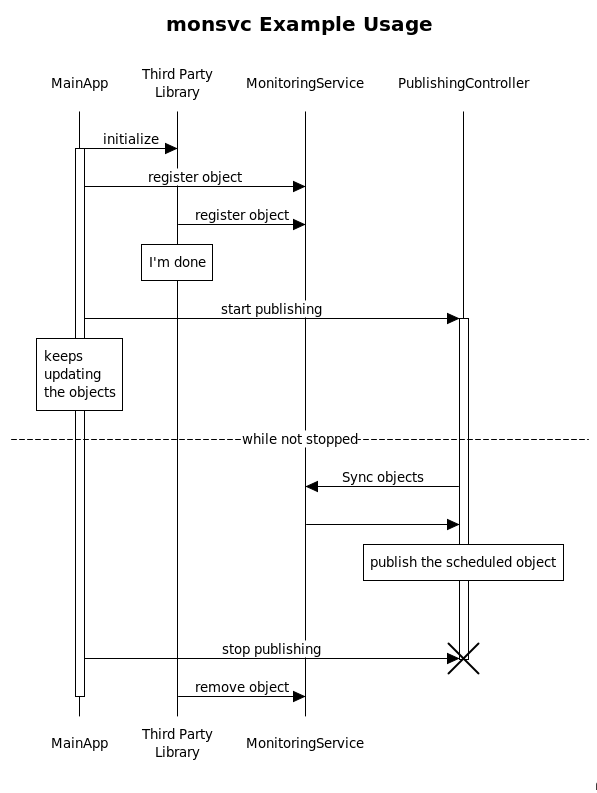
\includegraphics[scale=0.6]{Images/workflow.png}
\caption{{\tt monsvc} library usage example workflow.}
\end{figure}

The separation of registration and publishing also makes the life of third party library developers easier since their only job is to register the objects they want to be monitored while the main application is concerned with configuring and starting the publishing. For example, a network transport library will register information about the amount of trasferred data. This information will then be publsihed together with the main application data.

This usage pattern allows us to  create a lightweight version of the monsvc library with no transitive linking dependencies which contains only the registration functionality and which can be used by other libraries. The main application has to use the normal version which depends on a number of other packages like IPC, ROOT, IS, etc.


\chapter{Configuration} % Titlul capotilului
\label{Capitolul3}

\section{Introduction}

The applications in the ATLAS TDAQ system register up to several thousands of objects that represent information to be monitored. Different objects need to be published in different ways: for example with different publishing frequency and or to different Information Sharing (IS) servers or even need to be written to a file. As an example, the number of failed checksums of the event data read from the detector needs to be published every 10 seconds to an IS server called "L1". For another example, the histogram of accepted event data size should be written to a file called "DF.root" at the end of the running period. We aim to provide a way for the user to specify these parameters in an expressive, succinct and easy to use way. This process is called the \emph{configuration} of the library.

\section{Requirements}

The library allows the user to specify one or multiple \emph{publishing targets}. The publishing targets currently include IS servers, OH servers, files in ROOT format and standard output. For each target, the user can specify some \emph{publishing parameters}, for example, the name of the IS server and the publishing interval for an IS publishing target.

Another important functionality is to be able to modify the configuration at runtime. For example, if an operator notices some abnormal conditions in the running of the system, she may enable some debug monitoring information to be published in order to identify and fix the problem. 

\section{Challenges}

As with other parts of the system, the main challenge of the configuration is the scale of the system. We discuss below how each dimension of scaling impacts the design of the library.

\subsection*{The code size}

First of all, in order to publish a monitored object, the library needs to know the publishing parameters. The first decision to be made is whether to associate the parameters with the objects programmatically (in the source code), or in an external file which is loaded at runtime. We chose the second approach since, any change in the source code requires a recompilation and to create a binary patch of the current release version of the software. The duration and complexity of this process would discourage developers from changing configurations. In the external file approach, a change in configuration can be as simple as editing a text file and checking it in in the source repository.

\subsection*{The number of monitored objects}

With over 5000 monitored objects, we need to keep the configuration file of an application within a manageable size. We leverage the fact that the objects fall into a few semantic categories that share publishing requirements. We define groups of objects that share the same publishing parameters by using regular expressions. 

\begin{figure}[ht]
\centering
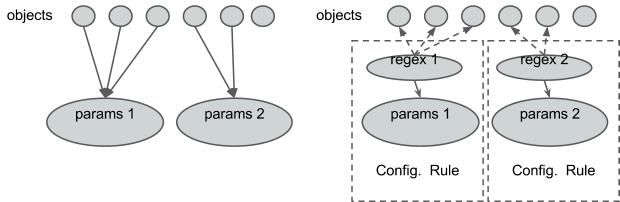
\includegraphics[scale=0.6]{Images/oks_regex.png}
\caption[Publishing parameters association.]{The two approaches for associating publishing parameters with monitored objects: explicit (left) and implicit by using regular expressions (right).}
\label{fig:oks_regex}
\end{figure}

As presented in the figure \ref{fig:oks_regex}, instead of having explicit links from the monitored objects to sets of parameters, we create links from parameters to objects by using configuration rules. A configuration rule is composed of a regular expression and a set of parameters. It is this rules that we store in the configuration file. A nice side-effect of this approach is that if the programmer registers a new object which uses an existing parameter set, she just has to give it a name that matches the regular expression.

One problem related to the object sets specification as regular expressions is that it is not easy to express exceptions from a rule. For example: we want to publish histograms with names matching {\tt “DEBUG/.*”} every 10 seconds, but we have a really big histogram among them that we would like to publish less often. To this end, we chose to add an exclude filter to every configuration rule that specifies the exceptions to that rule.

\subsection*{The number of developers}

In order to avoid complicated link time dependencies between packages, we adopted the split responsibility model: the developer of a library (other than {\tt monsvc}) registers some objects and the developer of the application (which uses the library) is the one who needs to configure their publishing parameters. Since some objects are registered by one developer and configured by another one, a clear convention should be used between the two. 

Our configuration mechanism allows the library developer to provide configuration rules for the objects registered by its library. To this end we created the concept of rule bundle which contains configuration rules and links other rule bundles. With this approach the developer of the main application can just link the rule bundle of the library from the rule bundle of the application. This mechanism handles nicely transitive dependencies by using transitively linked bundles.

The configuration files are a set of interlinked XML files, one per application or library. These files form the configuration database which can be loaded at run time by using the OKS system. The database is an object oriented one, where for example every application is described by a {\tt PublishingApplication} object which has a one to one relation to a rule bundle which is represented by an object of class {\tt ConfigurationRuleBundle}. The complete schema of the configuration database is presented in figure \ref{fig:oks_schema}. 

\begin{figure}[ht]
\centering
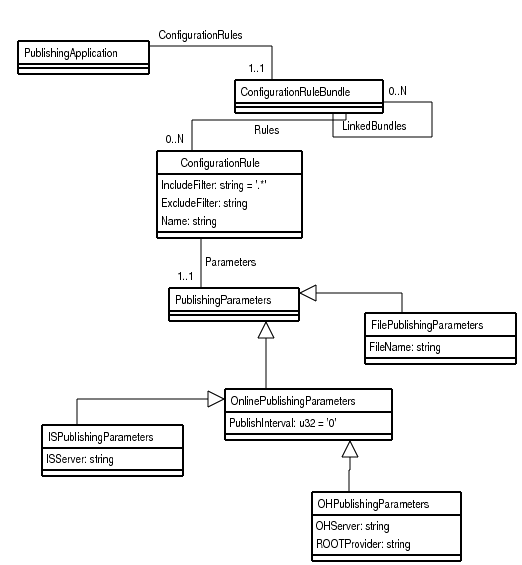
\includegraphics[scale=0.75]{Images/oks_schema.png}
\caption{Configuration database schema.}
\label{fig:oks_schema}
\end{figure}

\subsection*{The number of application instances}

Some applications in our system have several thousands of instances which use similar configuration files with only a few configuration parameters that differ. For example, if every application writes the objects in a file, then the name of the file should be different for the applications running on the same node. These configuration files are generated automatically from a common template using the partition editor tool.

Another challenge is related to the configuration changes during a running period. Our solution uses IS commands mechanism to allow the human operator to send the configuration change commands to the IS server which forwards them to the applications.

\chapter{Synchronization} % Titlul capotilului
\label{Capitolul5}

\section{Introduction}

As described in chapter \ref{Capitolul2}, the applications that use our library are take care of updating the monitored objects with the current operational values while in a separate thread the {\tt monsvc} library samples these objects and sends them to an IS server. Since some of the monitored objects are not thread-safe, for example ROOT histograms, this concurrent access pattern creates problems which include issues regarding visibility of updates of one thread in another one and accessing data structures in inconsistent state. Therefore, we need to synchronize the access to the monitored objects between application and library threads.

\section{Smart pointers}

We use smart pointers in order to implement the synchronization between the application and the library while requiring only minimal and incremental changes to the existing codebase. For every object registered with the library we return a smart pointer that is used by both library and application as a proxy for accessing the registered object. 

The smart pointers offer a simple interface to the application developer. They have two functions called lock and unlock which ensure exclusive access to the underlying object. Moreover, we use an interesting C++ feature \citep{andrei2001modern} that allows us to overload the dereference operator to lock the smart pointer just before any method call or field access and unlock it afterwards.

Due to the nice syntactical similarities between smart pointers and raw pointers we can easily port the code to use the former. It usually requires just changing the type of the declaration of the pointer. For example, the following function can be ported just by changing the type of the parameter:
\input{Code/dow1}
to obtain the following form:
\input{Code/dow2}
As explained above, the smart pointer takes care of the synchronization with the library on every function call and field access.

There is an exception to the previous case in which the pointer should be passed to a legacy function which we cannot change. For example:
\input{Code/dow3}
in which case we replace it with:
\input{Code/dow4}
Note that in this case even the change was very small, there is a trade-off between lock granularity and the amount of code that needs to be changed. For example, if we had ten calls to legacy functions and each of them was fast, we could as well lock around the \verb+do_work+ to save the refactoring work.

\section{Synchronization policies}

In the previous section we referred to locking and unlocking the smart pointer without giving details about how this is implemented. In this section we will present different implementations among which the application developer can choose when registering an object.

\subsection{No synchronization}

The information that is stored in the IS server is represented as objects with the base class ISInfo. Some of these objects are generated from XML description. We implemented a script which can generate a thread-safe version of the object which uses atomic integers for the fields. 

In cases where this level of thread-safety is sufficient, a developer can avoid the overhead of locking by using a smart-pointer that provides no synchronization.

\subsection{Mutex}

The simplest synchronization policy is to acquire mutex when accessing the object. The disadvantage of this policy is that the library has to lock the object while it sent over the network to the IS server. This is because the publishing to the IS server uses a legacy function similar with the example we have given before.

\subsection{Copy before publish}

When using this synchronization policy, the library makes local copy of the object before publishing it to the IS server. The advantage of this technique is that we avoid holding a lock while sending the object over the network. The disadvantage is that we consume more time and memory to make a copy of the object which may not be acceptable for large histograms.

This policy is the opposite of copy-on-write but we prefer it since in our case the object is written more often than is read.

\subsection{Asynchronous updates}

An important observation which we can leverage is that in our use cases, the application that updates an object with the current operational values does not need to wait for the update to be applied. All we are interested in is serial consistency of the operations on that object. 

With the asynchronous updates policy, we still use a mutex to ensure exclusive access to the underlying object. The only difference is that when the application tries to update a locked object it just enqueues the update to be applied at a later time. Our updates usually increment a counter or a histogram bin, hence they can be represented very compactly making this strategy lightweight in terms of space usage. It also avoid blocking the main application threads while sending the monitored objects over the network.

The interface of the smart pointer that implements this strategy leverages the C++11 variable argument templates to provides asynchronous updates to any type of monitored object. The declaration of the method responsible with asynchronous updates is the following:
\input{Code/async_ptr}

This method takes a pointer to a member function and its arguments and calls it asynchronously. It requires to change the method calls of the from \verb+h->observe(42)+ to use the following form: \verb+h.async(Histo::observe, 42);+.

Another positive point of this implementation is that we can rewrite only some of the method calls to be asynchronous, so there is again a trade-off between the amount of code to be modified and performance.

\subsubsection*{Intuition}

The figure \ref{fig:sync_ptr} represents the operation of the locking strategy while the figure \ref{fig:async_ptr} corresponds to the asynchronous updates strategy. One can see that in the second case, the application thread is not disturbed by the monitoring thread which is publishing the object that it is trying to update.
\begin{figure}[ht!]
\centering
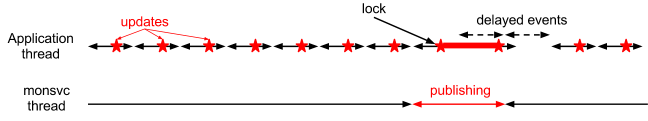
\includegraphics[scale=0.6]{Images/async_before.png}
\caption{Locking strategy}
\label{fig:sync_ptr}
\end{figure}

\begin{figure}[ht!]
\centering
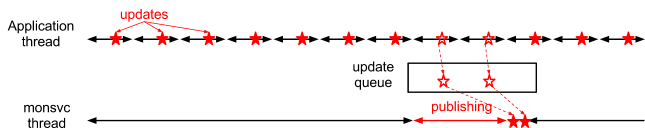
\includegraphics[scale=0.6]{Images/async_after.png}
\caption{Asynchronous updates strategy}
\label{fig:async_ptr}
\end{figure}

\subsubsection*{Implementation}

In this section we will present the implementation of the main operations of the smart pointer. The dereference operator is implemented on top of these operations. The smart pointer class has the following fields:
\begin{itemize}
\item {\tt update\_queue} the queue of updates that need to be executed asynchronously.
\item {\tt qlock} a mutex used to protect the {\tt update\_queue}.
\item {\tt obj\_lock} a mutex used to protect the object pointed by the smart pointer.
\end{itemize}
And the pseudocode is given below:
\input{Code/async}
Note that the {\tt async} method does not block when trying to acquire {\tt obj\_lock} since it uses the non-blocking {\tt try\_lock} method. 

Every thread that acquires the {\tt obj\_lock} mutex executes all updates that were added to the {\tt update\_queue} before accessing the underlying object of the smart pointer. This way we ensure that after the exclusive access to the object is given to the application, the object is in a serially consistent state. As an optimization, we also execute all updates before releasing the {\tt obj\_lock}.

\subsection{Custom mechanisms}

We also provide a smart pointer that uses callbacks to allow user to implement its own synchronization mechanisms such as, for example, per-cpu counters that are added up only before being read.

%% ----------------------------------------------------------------
\backmatter

\setstretch{0.9}  % Spatierea intre linii de 0.9 - o singura pagina de bibliografie
\addtocontents{toc}{\vspace{2em}}  % Spatiu in cuprins inainte de bibliografie

\label{Bibliografie}
\lhead{\emph{Bibliography}}  % Headerul paginii este "Bibliografie"
\bibliographystyle{unsrtnat}  % Stilul "unsrtnat"
\bibliography{bibliografie}  % Fisierul cu bibliografia

% Todo-uri in faza de lucru
%\todos
\end{document}
%% ---------------------------------------------------------------- 